
\par Biometria é uma característica física ou comportamental que identificam uma pessoa unicamente \cite{wayman2005biometric}. Desde suas descobertas e com o avanço tecnológico das últimas décadas, especialmente com os \textit{smartphones}, biometria têm ganho grande destaque na comunidade científica. Características biométricas como impressão digital, rosto e íris têm sido usadas em diversas aplicações, como controlar o acesso de pessoas em locais, controlar o acesso de pessoas em contas bancárias, confirmar pagamento e muitas outras \cite{wayman2005biometric, li2009encyclopedia}.

\par A íris é uma das características biométricas com maior confiabilidade, porque possui traços imutáveis ao longo da vida e diversos sistemas biométricos têm sido implementados as usando \cite{wayman2005biometric, daugman2004, iris_segmentada,othman2015}. No entanto, praticamente todos os sistemas usados comercialmente utilizam imagens com comprimento de onda \textit{\acrfull{NIR}}, que são adquiridas por meio de câmeras
especiais, e apesar de já ser utilizada por alguns \textit{smartphones} sofisticados, seus preços altos impossibilitam o uso de forma mais generalizada. Imagens de comprimento de \textit{\acrfull{LV}}, ou imagens tiradas por câmeras normais, como as
de \textit{smartphones}, também são utilizadas, mas não apresentam as mesmas taxas de eficiência das
imagens \textit{\acrshort{NIR}} \cite{trokielwicz2016-Warsaw, proenca2011,raja2014, raja2015}. Um dos fatores responsáveis pela menor taxa de acurácia pode ser explicado pela falta de controle na qualidade de imagens tiradas por câmeras normais, já que geralmente são tiradas pelas próprias pessoas e muitas vezes sobre condições desfavoráveis e porque imagens \textit{\acrshort{LV}} possuem algumas deficiências para capturar padrões da íris, especialmente de íris com pigmentação escuras \cite{abdullah2015}. 

\par Sistemas de reconhecimento de íris são implementados seguindo os três passos: segmentar e normalizar a íris; extrair atributos da íris segmentada e codificá-los, de forma a gerar o código de íris (\textit{IrisCode}); e comparar códigos gerados de forma a verificar se são ou não da mesma pessoa \cite{wayman2005biometric}. A etapa mais importante de sistemas de reconhecimento de íris é a segmentação, porque é nela que a íris é separada do restante da imagem de entrada e é utilizada para ser codificada \cite{daugman2004}. Muitas tentativas foram feitas para auxiliar os algoritmos de segmentação e, consequentemente, melhorar o desempenho de sistemas de reconhecimento de íris, como o cálculo da qualidade das imagens de íris de entrada do sistema \cite{daugman2004, starovoitov2013-DSMI-45, Jenadeleh_2018_CVPR_Workshops, wan2007-DSMI-50, bergmller2017-DSMI-2, chen2013-DSMI-4, kalka2010-DSMI-18, li2011} e o cálculo da qualidade da etapa de segmentação \cite{proenca2011, du2010, belcher2008, mottalli2009-DSMI-30, ma2003-FIM-7}, onde resultados que melhoraram o desempenho de sistemas de reconhecimento de íris foram encontrados para as duas abordagens. A métrica que apresentou o maior potencial e os melhores resultados para calcular a qualidade de imagens de íris \textit{\acrshort{LV}} foi o \textit{\acrfull{DSMI}} \cite{Jenadeleh_2018_CVPR_Workshops}, por considerar os ruídos mais comuns em imagens de íris, como os ilustrados na \refFig{fig:intro:ruidos}. Já para a qualidade da etapa de segmentação, a melhor métrica foi o \textit{\acrfull{FCE}} \cite{du2010} por levar em conta fatores como a qualidade dos padrões da íris, e fatores como ruídos e dilatação da pupila. No entanto, não foram encontrados projetos que calculam as qualidades da imagem de íris de entrada e da etapa de segmentação na mesma arquitetura do sistema de reconhecimento de íris.

\begin{figure}[h!]
\begin{subfigure}{.3\textwidth}
\centering
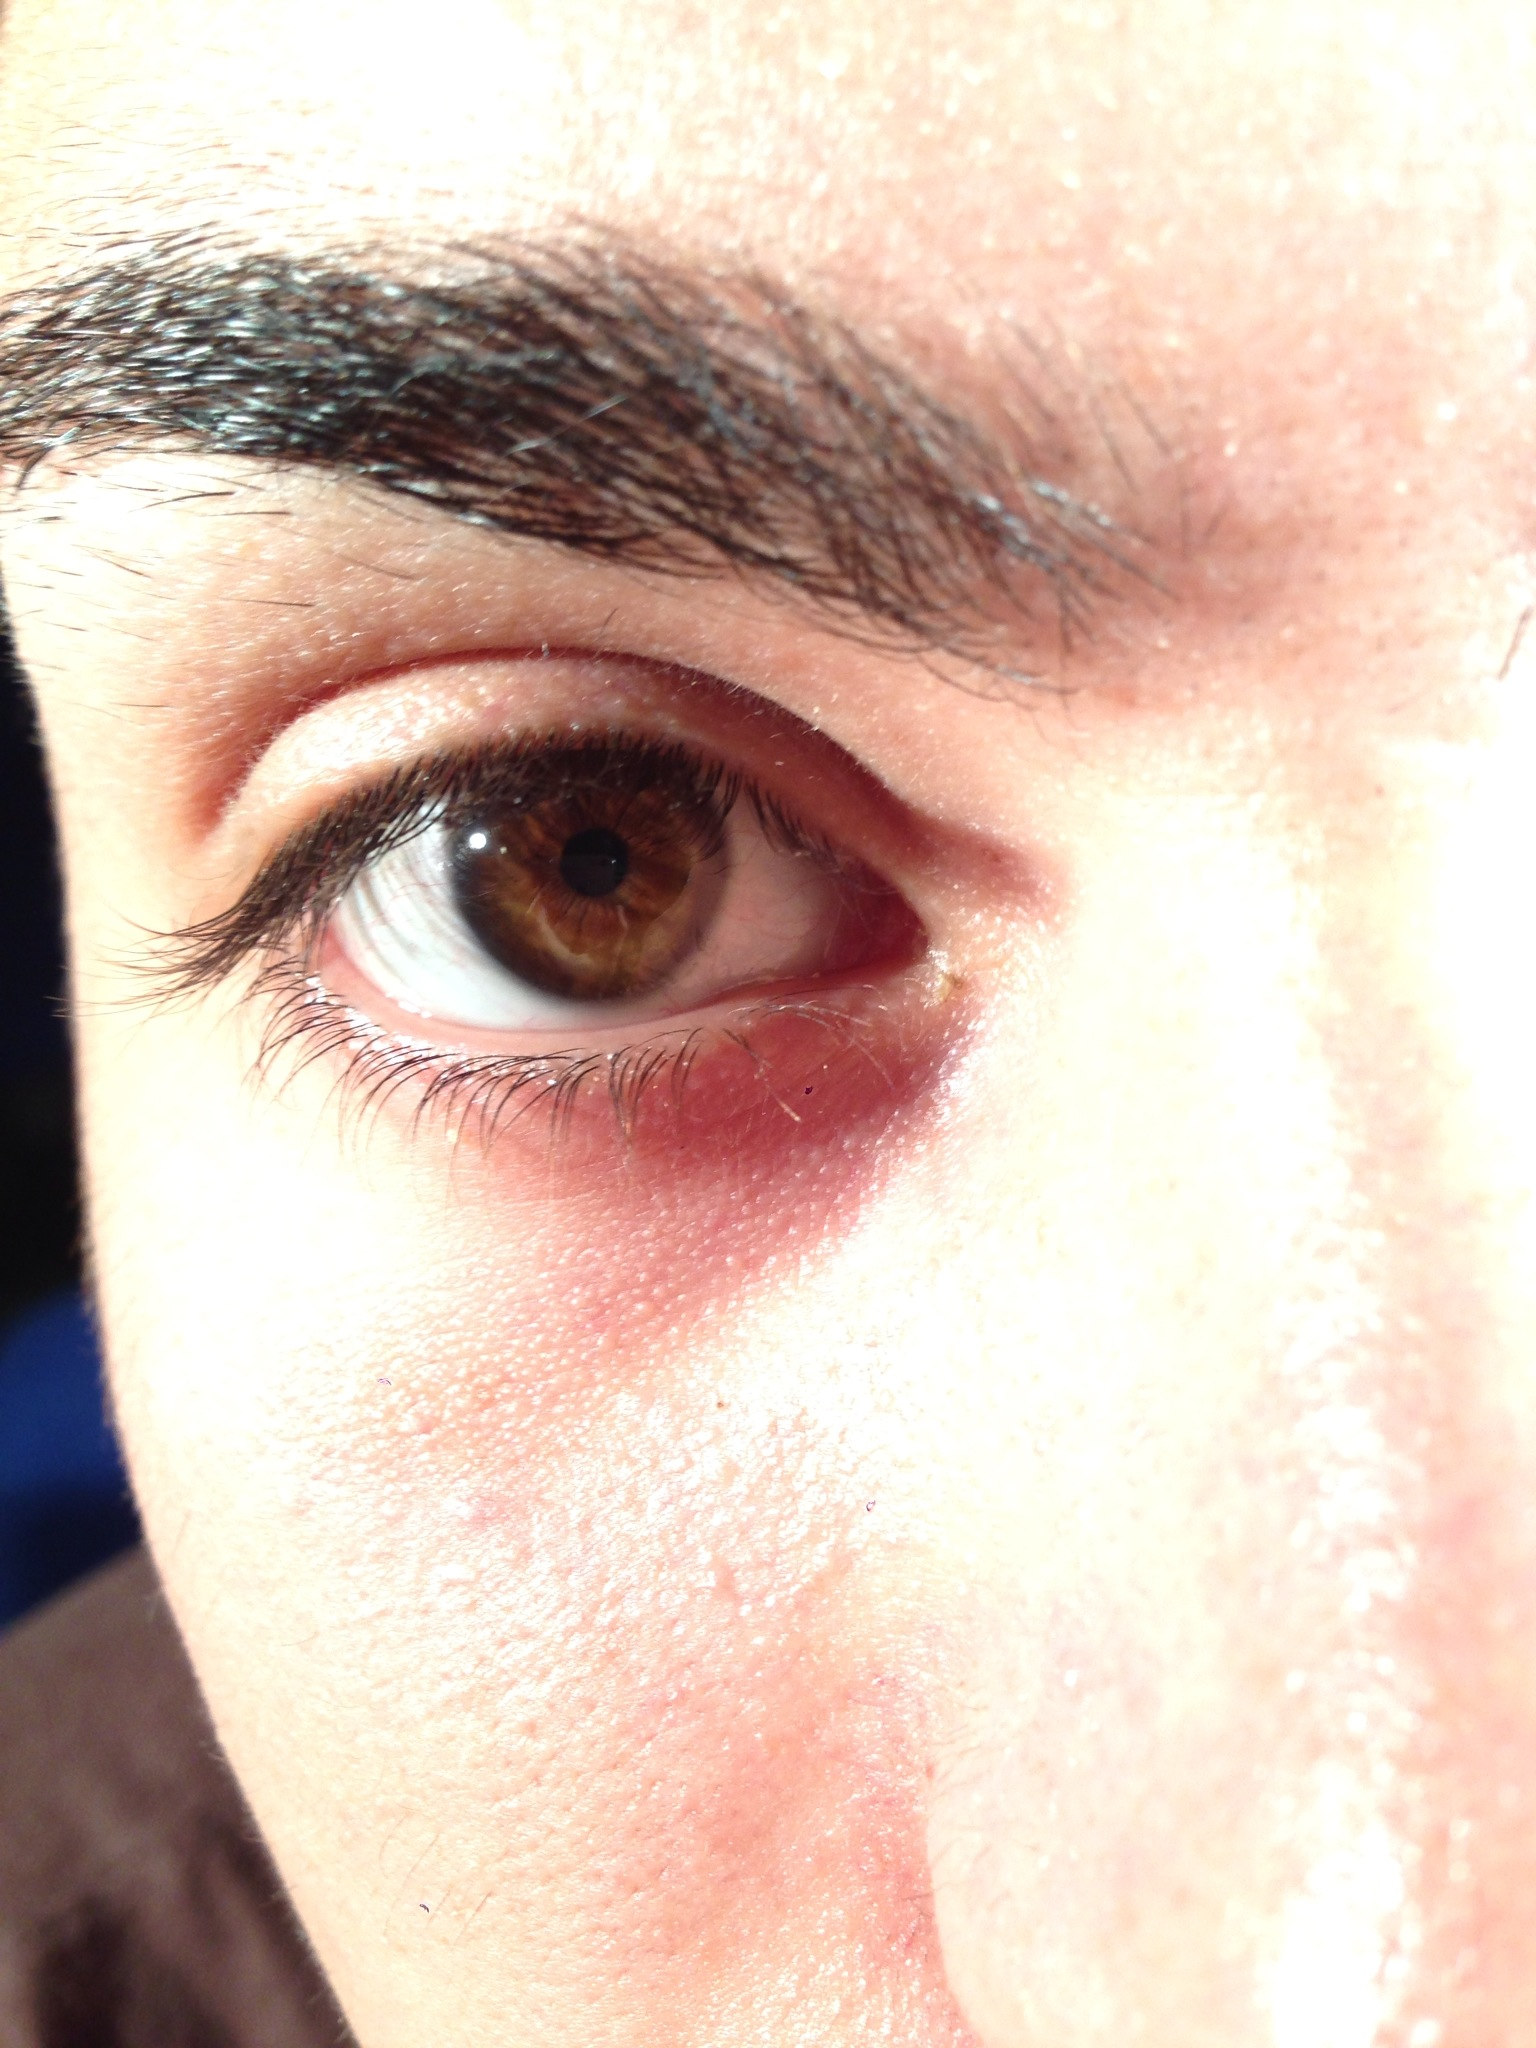
\includegraphics[width=4cm,height=5cm]{img/Resultados/miche/ruidosa.jpg}
\end{subfigure}\hfill
\begin{subfigure}{.3\textwidth}
\centering
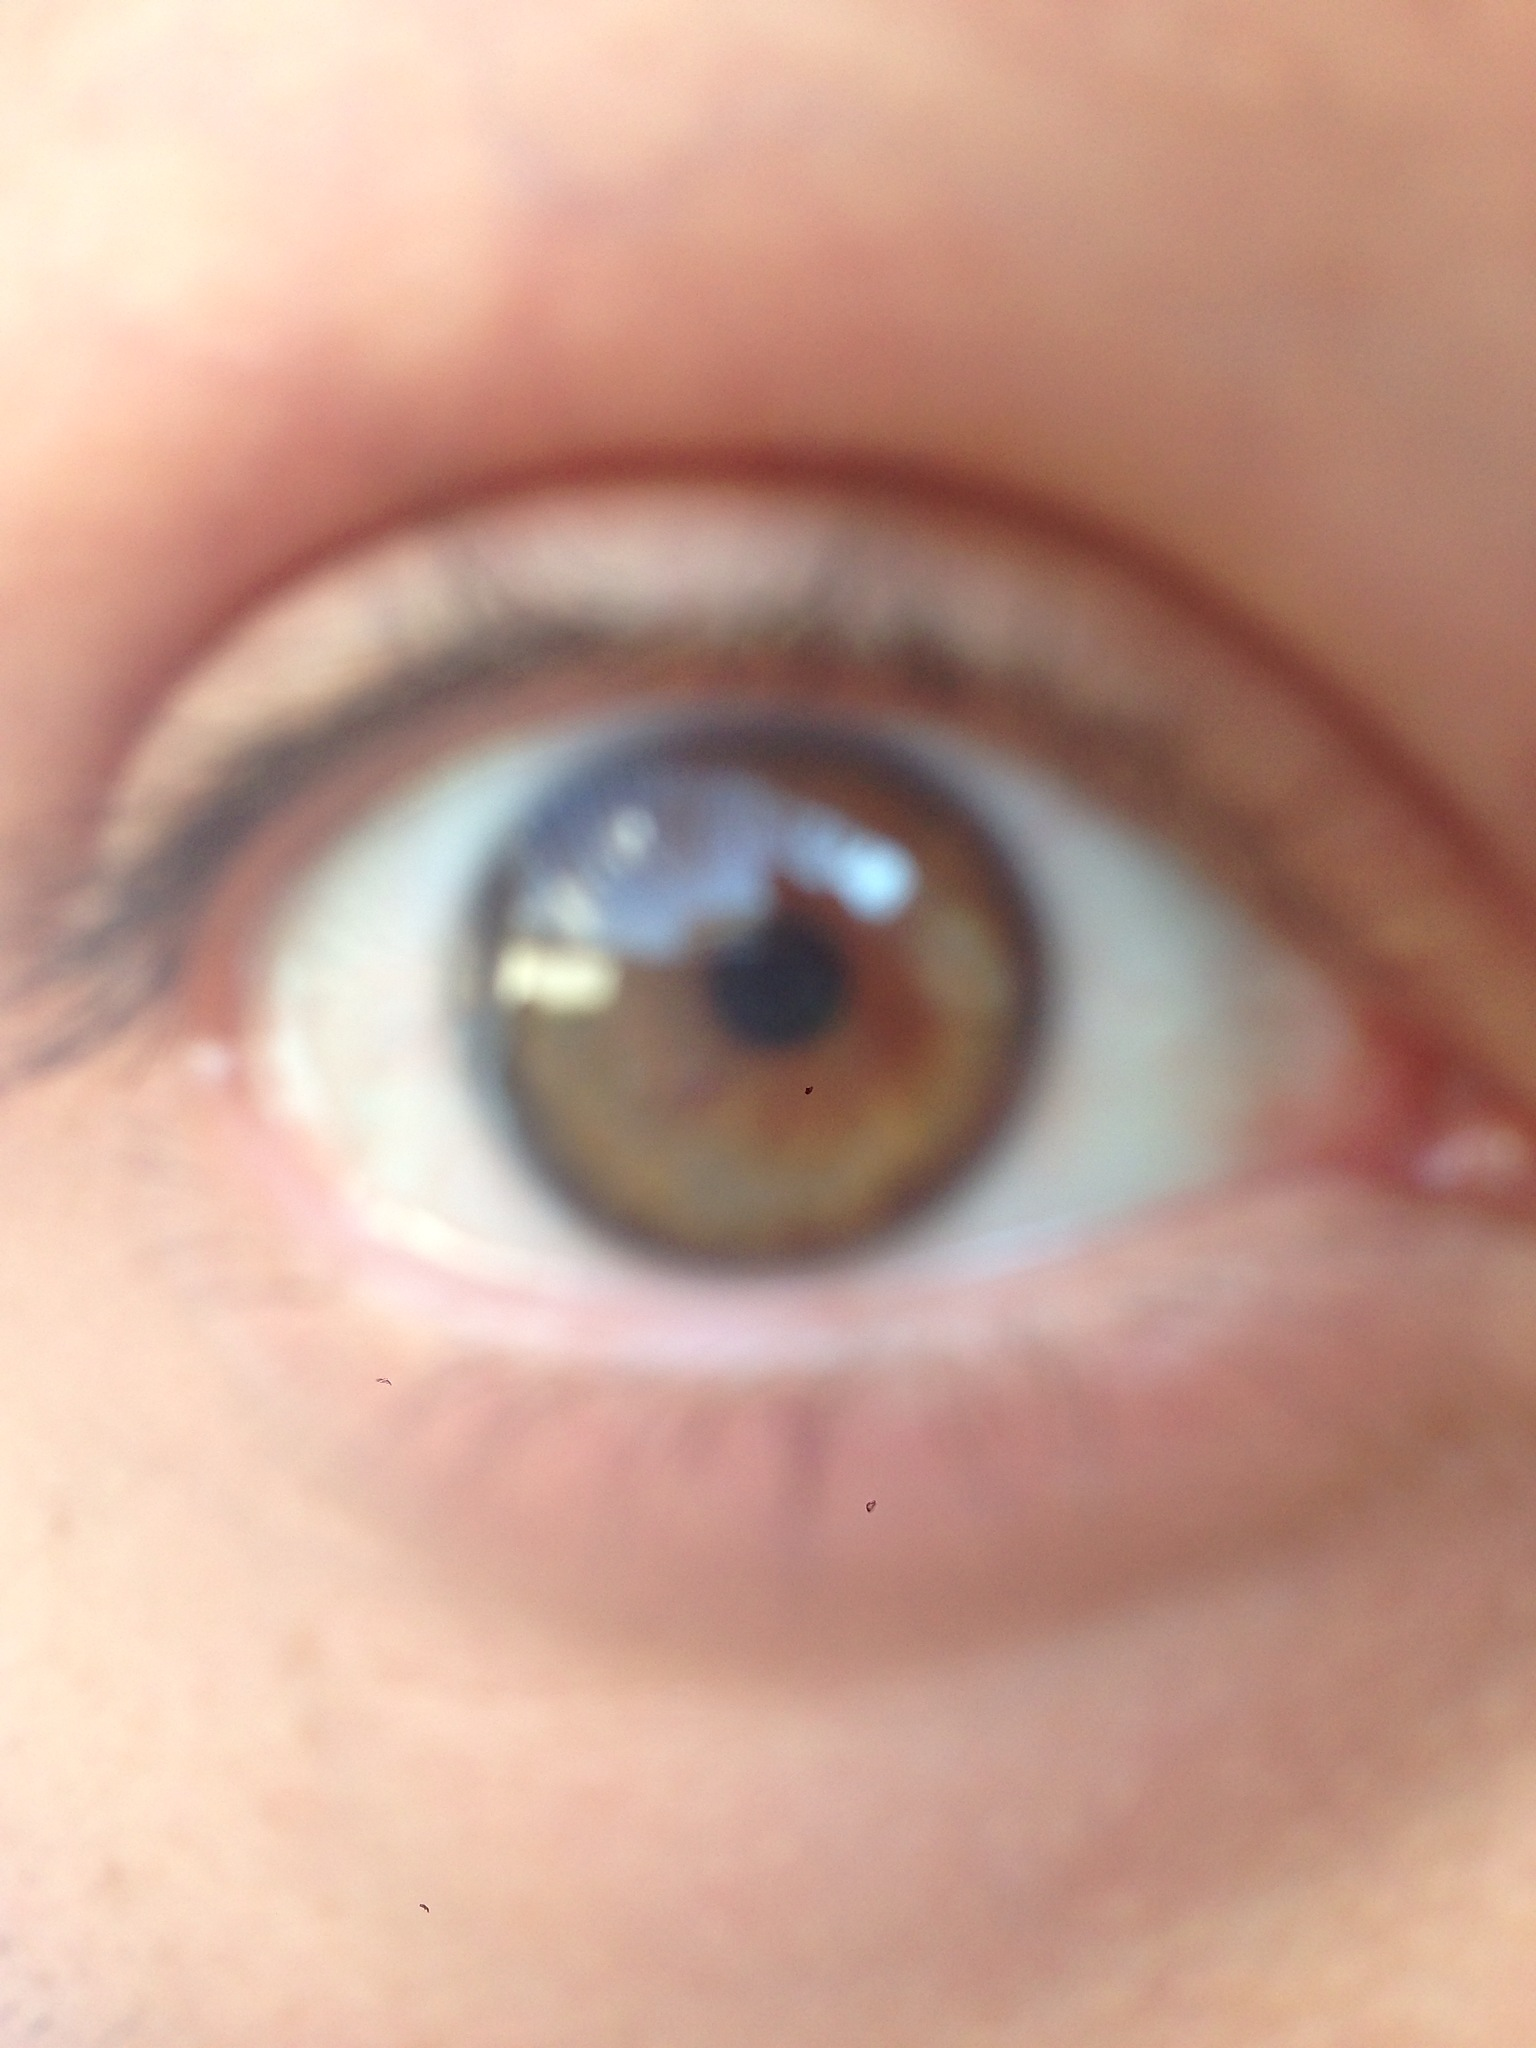
\includegraphics[width=4cm,height=5cm]{img/Resultados/miche/003_IP5_OU_R_RI_01_3.jpg}
\end{subfigure}\hfill
\begin{subfigure}{.3\textwidth}
\centering
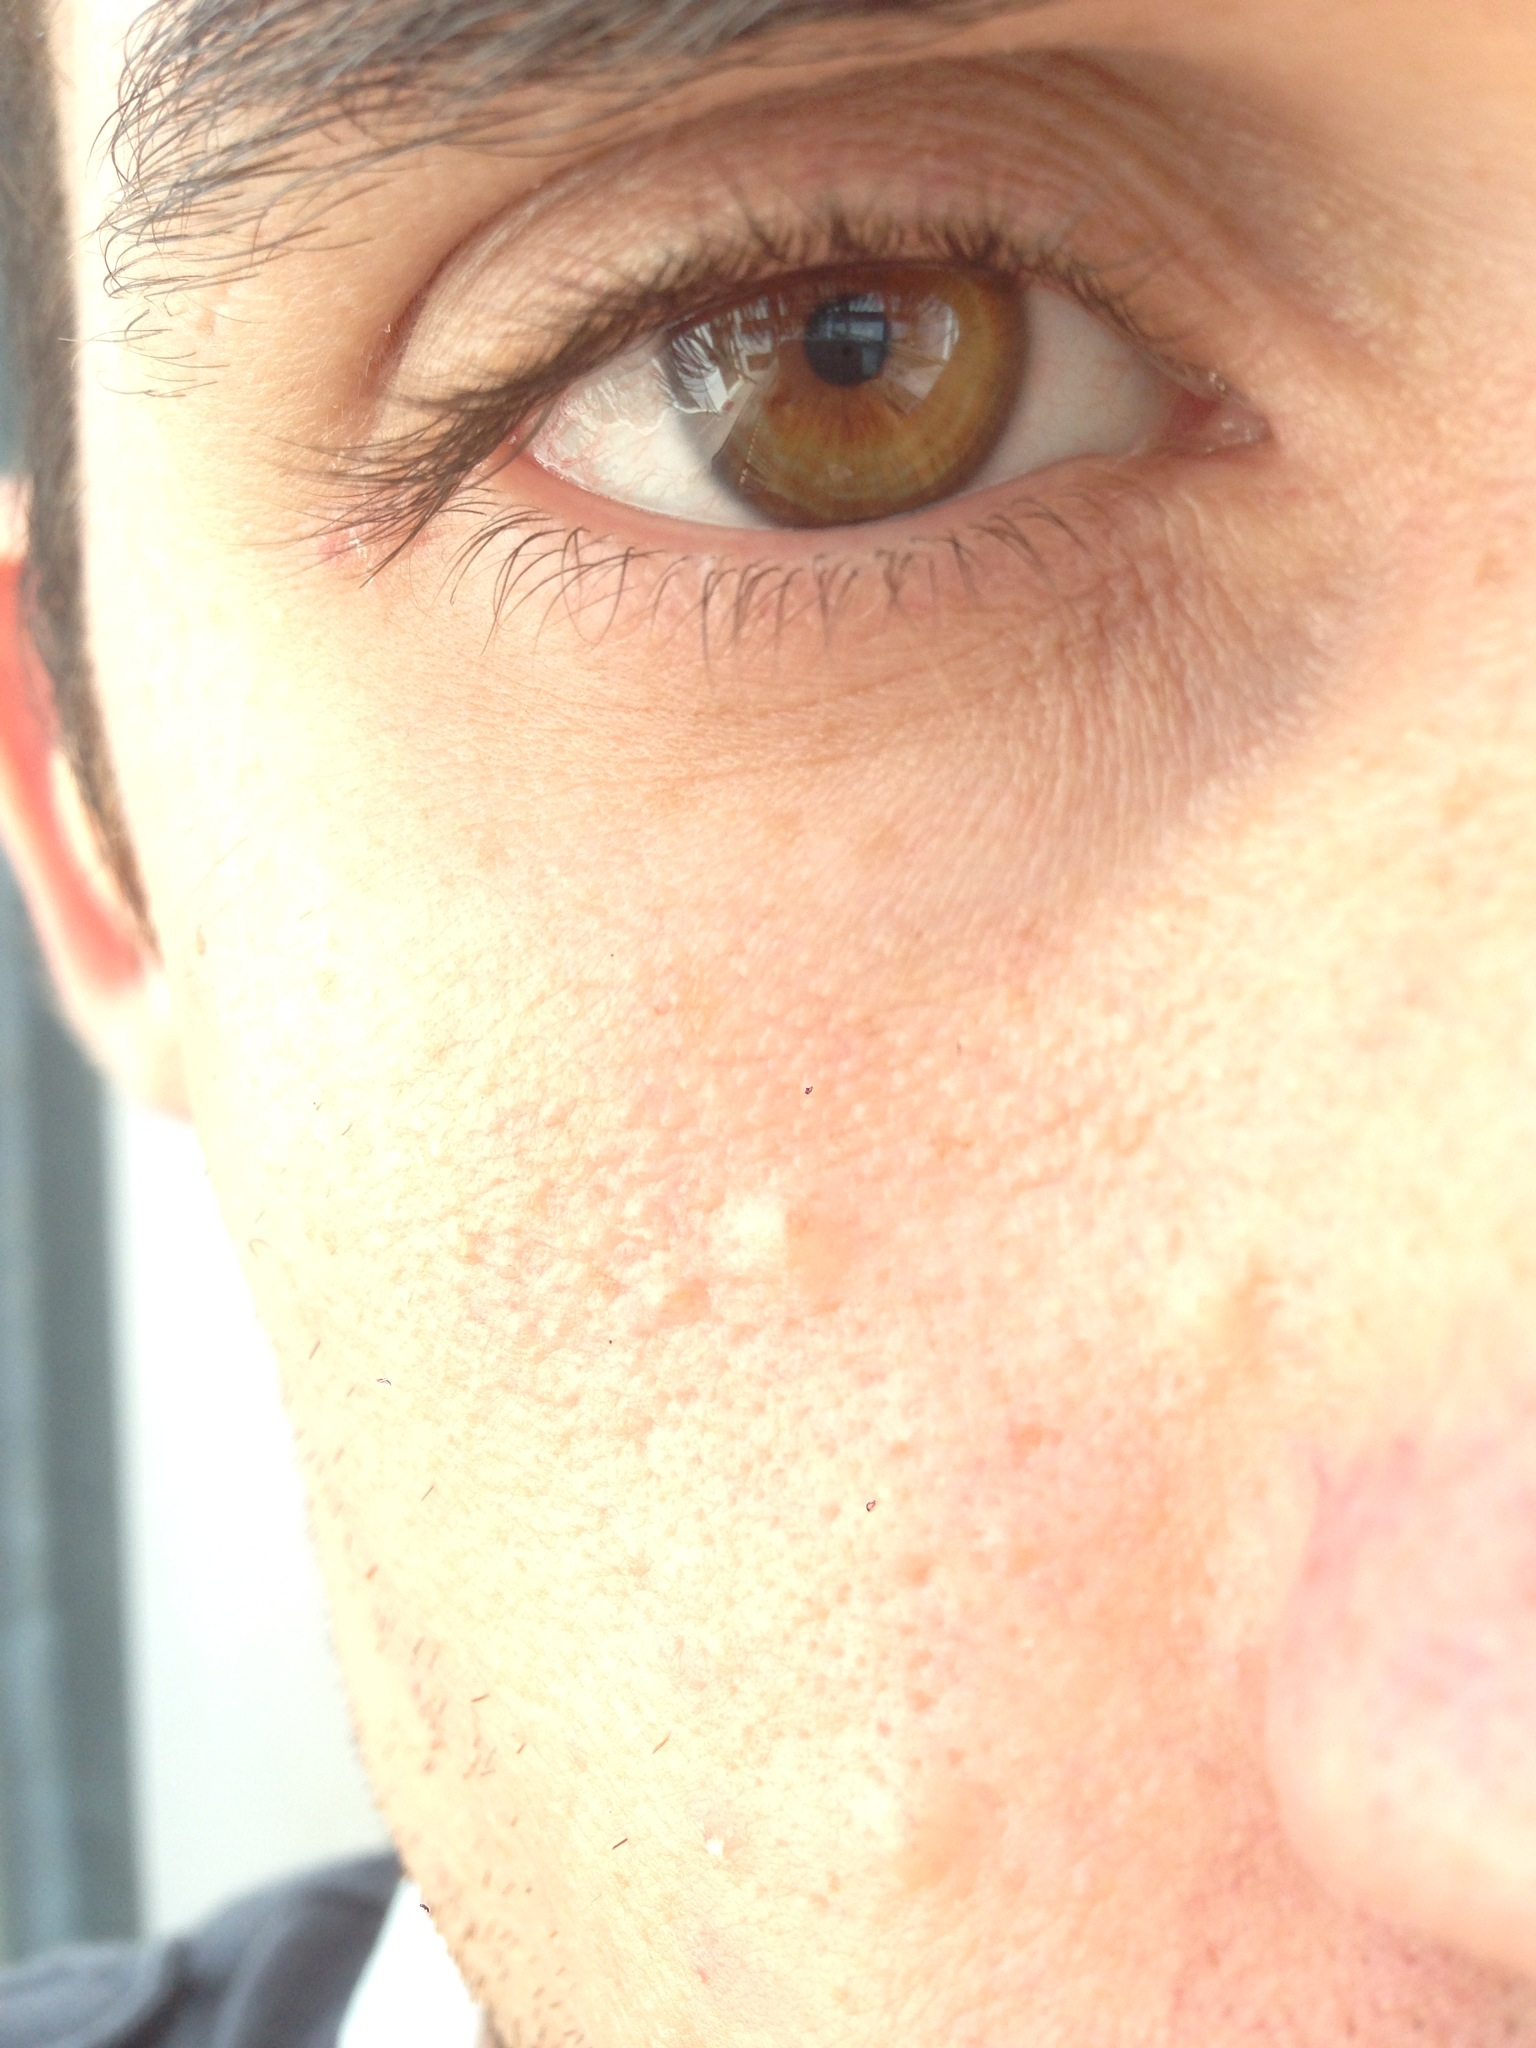
\includegraphics[width=4cm,height=5cm]{img/Resultados/miche/034_IP5_OU_R_RI_01_1.jpg}
\end{subfigure}
\caption{Ruídos comuns em imagens de íris.}
\label{fig:intro:ruidos}
\end{figure}

\section{Objetivo Geral}

\par Este projeto propõe uma arquitetura de sistema de reconhecimento de íris que utiliza duas métricas de qualidade: uma para avaliar a qualidade de imagens de íris \textit{\acrshort{LV}} (\textit{\acrshort{DSMI}}) e outra para avaliar a qualidade da etapa de segmentação de sistemas de reconhecimento de íris (\textit{\acrshort{FCE}}).

\section{Objetivos Específicos}

\begin{enumerate}
    \item Implementar as duas métricas de qualidade \textit{\acrshort{DSMI}} e \textit{\acrshort{FCE}};
    \item Propor uma arquitetura com as duas métricas de qualidade e flexível para usar qualquer sistema de reconhecimento de íris, ou seja, sistemas que implementam as etapas de segmentação, codificação e correspondência de íris. Neste projeto foi utilizado o sistema \textit{open source} \textit{OSIRISv4.1} \cite{othman2015};
    \item Avaliar como as duas métricas podem influenciar no desempenho de sistemas de reconhecimento de íris, utilizando quatro bancos de imagens com imagens de íris \textit{\acrshort{LV}}: \textit{MICHE} \cite{marsico2017-MICHE-1}, \textit{UBIRISv1} \cite{proenca2005-ubirisv1}, \textit{UBIRISv2} \cite{proence2010-ubirisv2} e \textit{\acrfull{Warsaw}} \cite{trokielwicz2016-Warsaw}.
\end{enumerate}


\section{Organização}

\par O \refCap{2_Fundamentacao} (Fundamentação Teórica) foi reservado para a introdução e explicação dos conceitos necessários para a melhor compreensão do projeto. No \refCap{3_Revisao} (Revisão Bibliográfica), é feita uma revisão de estudos e projetos que utilizaram os conceitos de qualidade de imagens, qualidade de imagens de íris e da etapa de segmentação de íris; além de explicar as métricas \textit{\acrshort{DSMI}} e \textit{\acrshort{FCE}}. O \refCap{4_Metodologia} (Metodologia) introduz e ilustra a arquitetura de sistema de reconhecimento de íris utilizando as duas métricas de qualidade proposta e explica cada um de seus módulos. O \refCap{5_Resultados} (Resultados) introduz os bancos de imagens de íris utilizados e todos os experimentos que foram realizados para avaliar o desempenho da arquitetura proposta. Por fim, o \refCap{6_Conclusao} (Conclusão) detalha as conclusões encontradas para o projeto proposto e analisa possíveis trabalhos futuros.